\documentclass[12pt,reqno]{amsart}

\usepackage{amsthm,amsmath,amssymb}
\usepackage{mathtools}
\usepackage{proof}
\usepackage{xcolor}
\usepackage{graphicx}
\usepackage[T1]{fontenc}
\usepackage{courier}
\usepackage{hyperref}
\hypersetup{
    hidelinks=true
}
\usepackage{listings}
\lstset{basicstyle=\ttfamily\small, columns=fullflexible, language=Lisp, morekeywords={define, lambda, if, car, cdr, zero, eopl}, keywordstyle=\bfseries\color{blue!40!black}}
\newcommand{\code}[1]{\texttt{#1}}
\graphicspath{ {./} }

\begin{document}

\begin{center}
\large\textbf{Problem Set 3 \\ COMP301 Fall 2019} \\
\normalsize\textbf{17.10.2019 17:30 - 18:45} \\
\end{center}

\vspace{7.5mm}

\textbf{Problem 1}\footnote{EOPL p.70 Exercise 3.4}: Write out the derivation of figure 3.4\footnote{EOPL p.66} in EOPL, as a derivation tree in the style of the one on EOPL p.5. \\

\vspace{4mm}

\begin{centering}
\frame{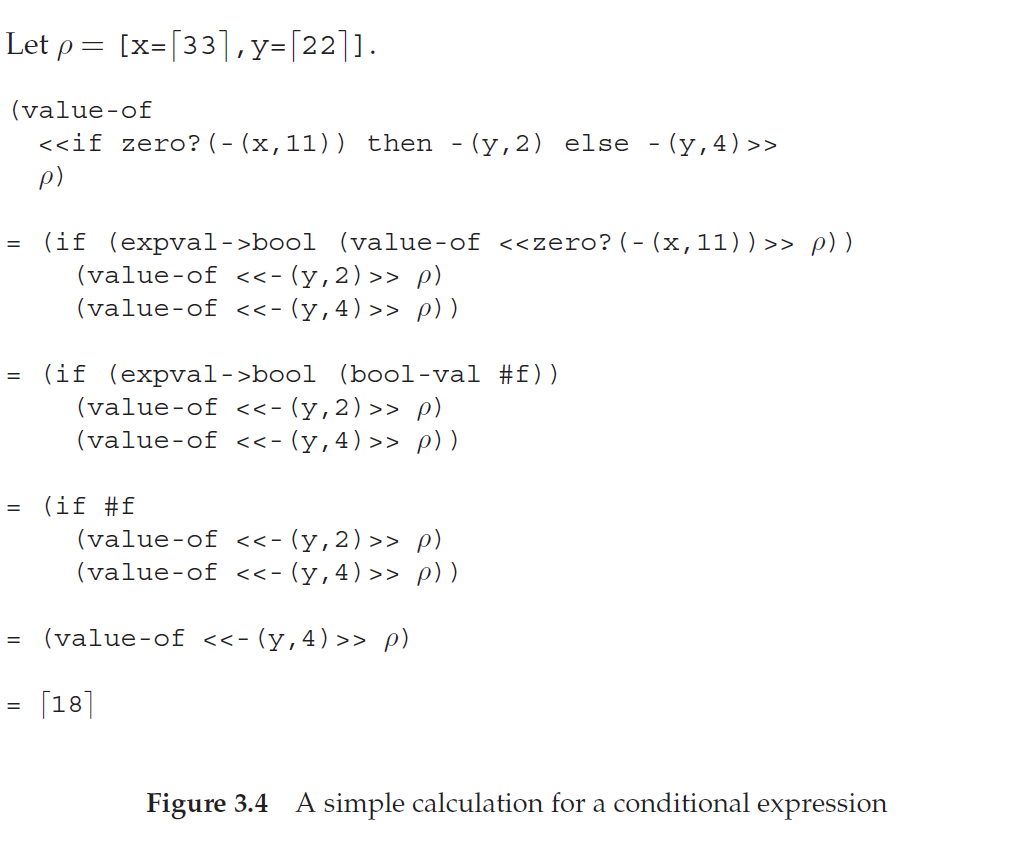
\includegraphics[width=\linewidth]{PS3Q2.PNG}}
\end{centering}
\newpage
\begin{figure*}
\label{FIG}
\caption{Rules of inference style, as seen on EOPL p.5}
\begin{centering}
\infer{\code{(-7 . (3 . (14 . ())))} }{
\infer{\code{(-7 . (3 . (14 . List-of-Int)))}}{
\infer{\code{(-7 . (3 . (Int . List-of-Int)))}}{
\infer{\code{(-7 . (Int . (Int . List-of-Int)))}}{
\infer{\code{(Int . (Int . (Int . List-of-Int)))}}{
\infer{\code{(Int . (Int . List-of-Int))}}{
\infer{\code{(Int . List-of-Int)}}{\code{List-of-Int}}
}
}
}
}
}
}
\end{centering}
\end{figure*}

\newpage
\textbf{Problem 2}\footnote{EOPL p.54 Exercise 2.27}:  Draw the abstract syntax tree for the lambda calculus expressions:
\begin{lstlisting}
((lambda (a) (a b)) c)

(lambda (x)
    (lambda (y)
        ((lambda (x)
            (x y))
        x)))
\end{lstlisting}

\vfill
\textbf{Please write \& draw your answers on a sheet of paper, then upload a readable photo or scan of that to the assignment on BlackBoard.}

\end{document}